\chapter{Introduction} \label{Introduction}
The first section of this chapter introduces the third generation light source BESSY II. The second section gives a brief overview over the Variable Pulse Length Storage Ring project (\textit{VSR}). The challenge of the cavities' installation length is showcased in the third section and is the motivation of this thesis.

\section{BESSY II - A third generation light source}
\begin{figure}
	\centering
	\includegraphics[width = \textwidth]{images/01-BESSY-II-floor-plan.pdf}
	\caption[Floor plan of synchrotron light source BESSY II.]{Floor plan of synchrotron light source BESSY II (extracted from~\cite{Rubrecht_PhD}).}
	\label{fig:Bessy2-plan}
\end{figure}
\begin{table}
	\centering
	\footnotesize
	\caption{Parameters of the BESSY II storage ring.}
	\begin{tabular}{ll}
\toprule
\textbf{Parameter}  &  \textbf{Value}\\
\midrule
nominal energy & 1.7\,GeV\\
circumference & 240\,m\\
RF-frequency & 500\,MHz\\
revolution time & 800\,ns\\
beam current & 300\,mA\\
number of cells & 16\\
number of bending magnets & 32\\
bending radius & 4.361\,m\\
beamlines & $\approx$ 50\\
\bottomrule
\end{tabular}

	\label{tab:mostimportantparameter}
\end{table}

The third generation synchrotron light source BESSY II is located in Berlin Adlershof and is operated by the research institute HZB since 1998. Its purpose is to provide extremely brilliant synchrotron light pulses in the range from long terahertz radiation to hard X-rays. The storage ring has a circumference of 240\,m and is equipped with 50 beamlines. A graphic overview of BESSY II is shown in \autoref{fig:Bessy2-plan}. The most important parameters of the storage ring are listed in \autoref{tab:mostimportantparameter}.

The electrons are emitted by a DC grid cathode and are accelerated up to 90\,keV. In the following linac their energy is increased up to 50\,MeV~\cite{linac}. Next the electrons are transfered to the booster synchrotron, where they are accelerated up to 1.7\,GeV and are than injected to the storage ring cumulatively, so that a beam current of 300\,mA is maintained (\textit{top-up}). The electrons can be saved for up to 10 hours and emit, depending on the type of deflection (bending magnet, wiggler or undulator), photon energies up to 15\,keV.

At BESSY II it is possible to operate the machine in two different modes. Most of the time the storage ring is set to the standard user optics with 15\,ps bunch length. During two weeks of the year the lattice is changed to the low alpha optics, which provide buckets with 3\,ps bunch length~\cite{vsrstudy}. This can be realized by reducing the momentum compaction factor $\alpha_{\textup{c}}$ from  $7 \cdot 10^{-4}$ to $4 \cdot 10^{-5}$. The coherent synchrotron radiation instability leads to a limiting bursting threshold current, which scales with~$\alpha_{\textup{c}}$. Therefore the photon flux has to be reduced significantly in comparison to the standard optics. In this time high flux user are not able to run experiments, which is the reason that the low alpha mode can only be provided for short periods.

%Independent of the optics the 400 available buckets of the storage ring can be filled with different patterns. In the multibunch mode the 300-350 buckets are filled. This allows for a high beam current with high brightness. In the single and few bunch mode the electron bunch charge is increased up to 100\,nC. As there is no emission for a relatively long period of about 800\,ns this allows especially for time-resolved experiments.


\section{Overview of the BESSY-VSR project}
%Due to the increasing user demands the facility BESSY~II was undergoing many modification within the last several years. 
Currently, there is a continuously increasing interest in the short pulse operation from the user community. Therefore the next major upgrade BESSY-VSR aims to provide short intense pulses by storing short and long pulses in one storage ring, simultaneously~\cite{vsrstudy}. This variable pulse-length storage ring can be achieved due to the installation of additional cavities. The superposition of the 0.5\,GHz, 1.5\,GHz and 1.75\,GHz cavity voltages, shown in \autoref{fig:cavity-voltage}, changes the 400 equal buckets of BESSY~II to a bunch length scheme, where long and short buckets alternate.

The long bunches are located at the small voltage gradients, where the voltages of the 1.5\,GHz and 1.75\,GHz cavities cancel out. The short bunches, with higher current than in the low alpha mode, are produced at the high voltage gradient, where the voltages of the cavities add up. This fulfills the requirements of the users which need short 2\,ps bunches and of the users relying on the high average beam current, which is mainly stored in the 15\,ps long bunches. The goal of BESSY-VSR is to maintain the current beam quality and adding a new flexibility for user experiments.
\begin{figure}
	\centering
	\includegraphics[width = 0.9\textwidth]{images/01-cavity-voltage.pdf}
	\caption[Superposition of the cavity voltages for BESSY-VSR.]{Superposition of the cavity voltages for BESSY-VSR (based on~\cite{Rubrecht_PhD,vsrstudy}). The large slope at $t=\SI{0}{\nano\second}$ and $t=4$\,ns generates short bunches. The small slope at $t=2$\,ns leads to long bunches.}
	\label{fig:cavity-voltage}
\end{figure}


\section{Motivation of this thesis: The challenge of the cavities' installation length}
Two 1.5\,GHz and two 1.75\,GHz cavities will be assembled into one cryomodule in the T2 section of the storage ring. This module needs more space than initially assumed. The T2 section of the storage ring is shown in \autoref{fig:cavity-in-T2}. The idea is to remove the two Q5T2 magnets to gain installation length. According to the simulation lattice files the two quadrupoles and the adjoining drift spaces have a length of 70,6\,cm. Due to coils and connection elements the effective gain of installation length amounts to 66,0\,cm.

Before the Q5T2 magnets in the storage ring lattice can be removed, the influence on the beam dynamics has to be investigated in simulations. The orbit of an accelerator is defined by the position and strength of its bending magnets. The motion of particles with a small spatial offset is largely dominated by the linear order multipole terms. Higher order multipoles are used for the compensation of higher order effects and have not been taken into account in this thesis. Hence for fundamental lattice design and optimization tasks the optics has first to be optimized in regards to the linear order.

To compensate the switch off of the Q5T2 quadrupoles the other quadrupoles have to be adjusted. Thereby the goal should be to maintain the most important transverse linear beam parameters as the beta functions, the tunes or the momentum compaction factor. An introduction into transverse linear beam optics in circular accelerators is provided in the next chapter.


\begin{figure}
	\centering
	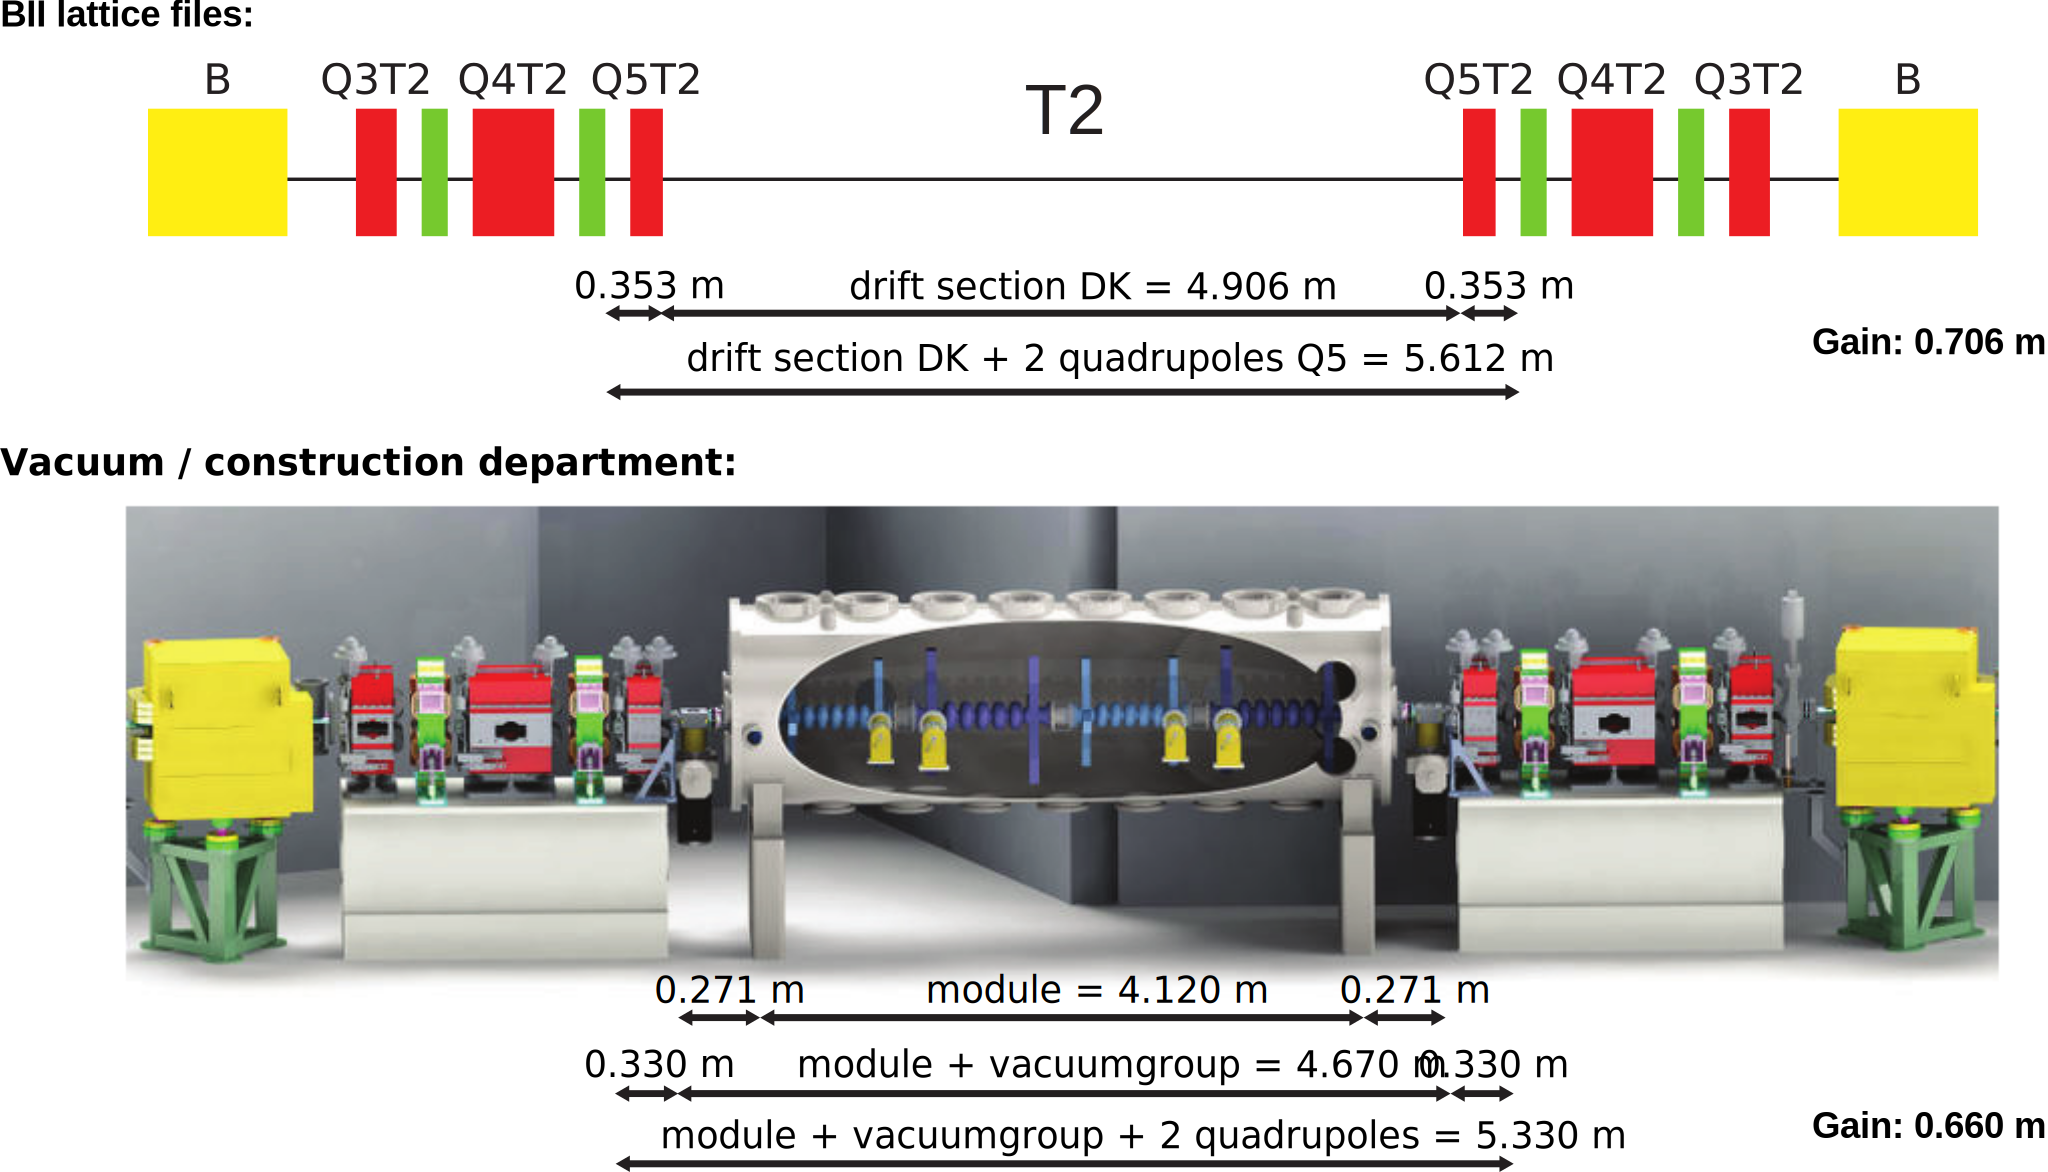
\includegraphics[width = \textwidth]{images/01-cavity-in-T2.pdf}
	\caption[The cryomodule and the magnets of the T2 section.]{The cryomodule and the magnets of the T2 section (dipole-yellow, quadruple-red, sextupole-green).}
	\label{fig:cavity-in-T2}
\end{figure}